\chapter{Обобщенная модель Изинга на квадратной решетке}\label{ch:ch4}

Первой работой по обобщению модели Изинга на несколько трансляций решетки была статья Утиямы~\cite{utiyama1951} на примере шахматной решетки, в которой все черные квадраты замещаются специальными вставками~(рисунок~\ref{utiyama}). В случае, когда $n=0$, что означает всего один квадрат в качестве вставки со взаимодействиями $J, J_1$ и $J_0$, можно получить квадратную необобщенную, треугольную и гексагональную решетки. Положив $n=1$, получим решетку кагоме (в качестве вставки два квадрата со взаимодействиями $J, J_0, J_1, J_2, J_3$) и устремив $J_1$ к нулю (рисунок~\ref{ut}). Таким образом, обобщение модели Изинга при больших $n$ дает колоссальное количество новых еще неисследованных решеток.

% \begin{figure}[h]
% 	\center{\includegraphics[width=0.6\linewidth]{Pictures/fig4.eps}}
% 	\caption{Обобщение модели Изинга, предложенное Утиямой, на шахматной решетке}
% 	\label{utiyama}
% \end{figure}

% \begin{figure}[h]
% 	\begin{minipage}{0.45\linewidth}
% 		\center{\includegraphics[width=1\linewidth]{Pictures/fig5(a).eps} \\ а)}
% 	\end{minipage}
% 	\hfill
% 	\begin{minipage}{0.45\linewidth}
% 		\center{\includegraphics[width=1\linewidth]{Pictures/fig5(b).eps} \\ б)}
% 	\end{minipage}
% 	\caption{Переход от решетки Утиямы ($n=1$) к решетке кагоме: а) Решетка Утиямы с одной вертикальной чертой при $J_1 \rightarrow 0$, б) Решетка кагоме}
% 	\label{ut}
% \end{figure}

Следующими работами по обобщению модели Изинга стали статьи Сиози и Найя~\cite{syozi1960} (см. также~\cite{siozi_domb1972}). В этих работах авторы приводят точное аналитическое решение обобщенной модели Изинга на квадратной решетке с двумя трансляциями в горизонтальном ($J_{2}, J_{4}$) и вертикальном ($J_{1}, J_{3}$) направлениях~(рисунок~\ref{gen}). Синими прямыми указаны связи между соседними спинами по горизонтальному направлению с обменным взаимодействием $J_1$, синими пунктирными линиями по горизонтальному направлению  --- $J_3$, красными прямыми линиями по вертикальному направлению --- $J_2$, красными пунктирными линиями по вертикальному направлению --- $J_4$. Обратим внимание, что помимо точного решения исследований каких-либо термодинамических и фрустрационных свойств не проводилось.

Главным преимуществом обобщенной решетки является то, что из структуры такого типа обобщения можно получать различные виды других решеток с помощью предельных переходов. Например, при $J_1 = J_3$ и $J_2 = J_4$ решетка сводится к обычной квадратной решетке, решение которой рассмотрено в Главе 1. Так же может быть осуществлен переход к гексагональной решетке. Для этого необходимо устремить к нулю одно из четырех обменных взаимодействий, например, $J_4 \rightarrow 0$. Получаемая таким образом решетка типа \guillemotleft кирпичная кладка\guillemotright$ $ (brick-wall lattice), показанная на рисунке~\ref{hex}, топологически эквивалентна гексагональной решетке. В случае же перехода к треугольной 

% \begin{figure}[H]
% 	\center{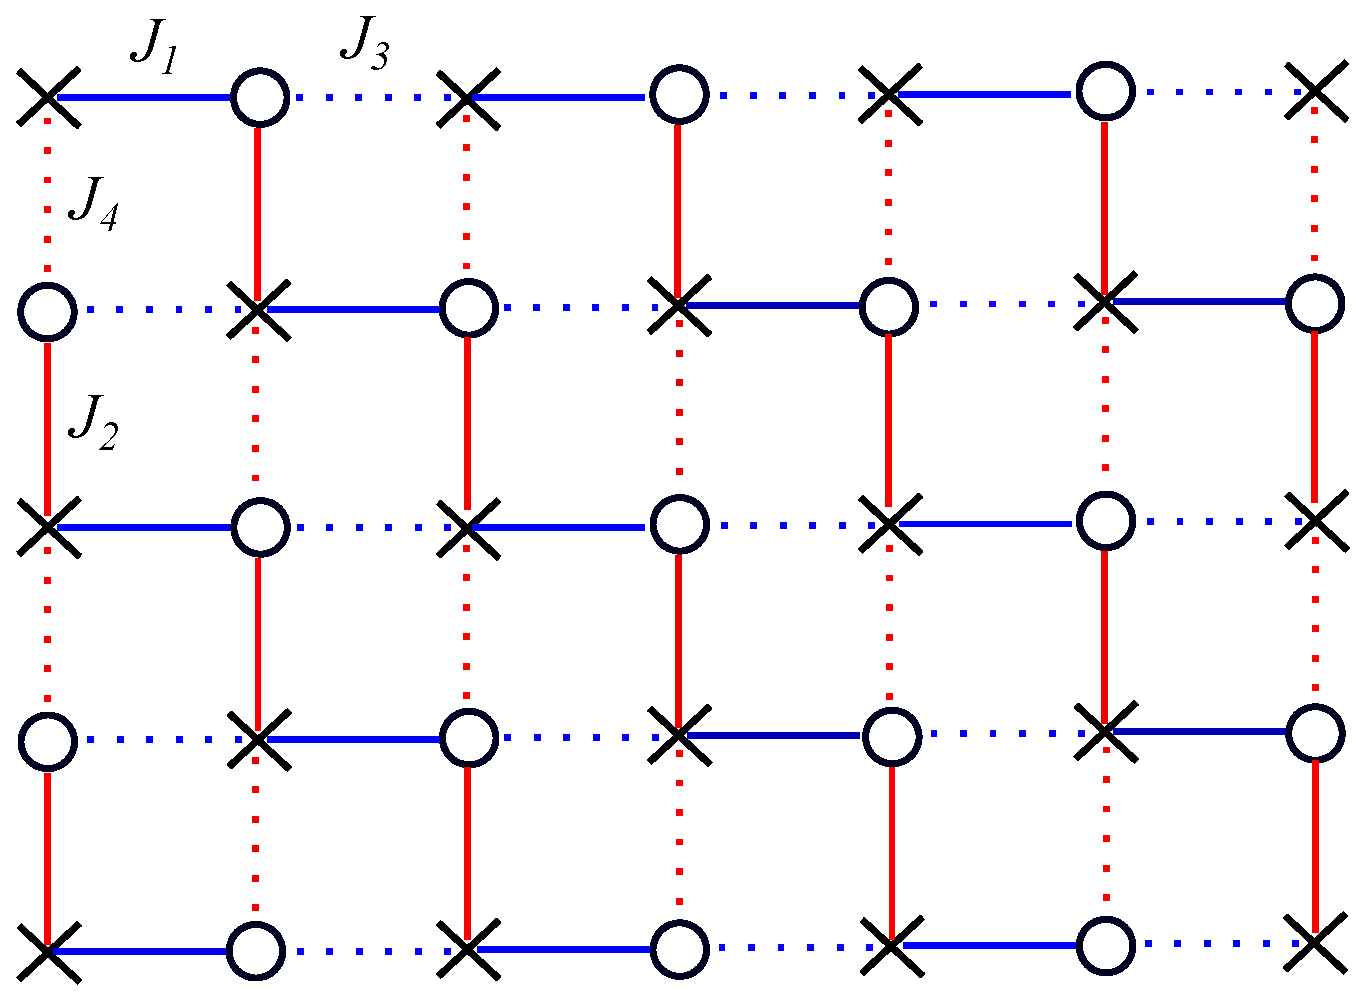
\includegraphics[width=0.6\linewidth]{New_figure/gen.eps}}
% 	\caption{Обобщенная квадратная решетка}
% 	\label{gen}
% \end{figure}

\noindent решетке, одно из четырех обменных взаимодействий обобщенной модели устремляется в бесконечность, например, $J_1 \rightarrow \infty$, (см. рисунок~\ref{triag}).

Очевидно, что данные варианты обобщения, введенные на квадратной решетке Утиямой, Сиози и Найя, могут быть применены и к другим планарным решеткам с известными точными решениями (треугольная~\cite{wannier1950}, гексагональная~\cite{houtapell1950}, кагоме~\cite{kano_naya1953}). В результате, всевозможными вариантами предельных переходов осуществляется получение множества самых разнообразных видов еще неизученных решеток.

% \begin{figure}[h]
% 	\center{\includegraphics[width=1\linewidth]{New_figure/hex.eps}}
% 	\caption{При $J_4 = 0$ обобщенная квадратная решетка превращается в так называемую кирпичную кладку, которая топологически эквивалентна гексагональной решетке}
% 	\label{hex}
% \end{figure}

% \begin{figure}[h]
% 	\center{\includegraphics[width=1\linewidth]{New_figure/triag.eps}}
% 	\caption{Переход от обобщенной квадратной решетки к треугольной решетке при $J_1 \rightarrow \infty$}
% 	\label{triag}
% \end{figure}

В настоящей магистерской диссертации рассматривается модель Изинга на обобщенной квадратной решетке (рисунок \ref{gen}), с последующим изучением ее термодинамических и фрустрационных свойств. 


\section{Точное решение обобщенной модели Изинга на квадратной решетке}

Получим точное аналитическое решение обобщенной модели Изинга на квадратной решетке комбинаторным методом Вдовиченко--Фейнмана.

Статсумму приведенной решетки можно представить следующим образом 
\begin{multline}
Z_{N} = \sum_{\{\sigma\}} \exp{\bigg[ K_1 \sum_{\substack{i = 1,3,\dots \\ j = 2,4,\dots}} \sigma_i \sigma_j + K_2 \sum_{\substack{i = 2,4,\dots \\ k = 3,5,\dots}} \sigma_i \sigma_k + }\\{ +  K_3 \sum_{\substack{i = 2,4,\dots \\ j = 3,5,\dots}} \sigma_i \sigma_j + K_4 \sum_{\substack{i = 1,3,\dots \\ k = 2,4,\dots}} \sigma_i \sigma_k\bigg]},
\end{multline}
где первая и третья суммы идут по половинам спинов в горизонтальном направлении,  а вторая и четвертая суммы идут по половинам спинов в вертикальном направлении, так что
\begin{equation*}
K_1 = \frac{J_1}{T}; \;\;\;\;\;\; K_2 = \frac{J_2}{T};\;\;\;\;\;\; K_3 = \frac{J_3}{T};\;\;\;\;\;\;K_4 = \frac{J_4}{T}.
\end{equation*}

Перепишем статсумму в виде
\begin{align}
&Z_{N} = (\ch K_1 \ch K_2 \ch K_3 \ch K_4)^N S, \nonumber \\
&S = \sum_{\{\sigma\}} \prod_{\substack{i = 1,3,\dots \\ j = 2,4,\dots}} (1 + v \sigma_i \sigma_j) \prod_{\substack{i = 2,4,\dots \\ k = 3,5,\dots}} (1 + u \sigma_i \sigma_k) \times \nonumber\\&\;\;\;\;\;\;\;\;\; \times \prod_{\substack{i = 2,4,\dots \\ j = 3,5,\dots}} (1 + w \sigma_i \sigma_j) \prod_{\substack{i = 1,3,\dots \\ k = 2,4,\dots}} (1 + t \sigma_i \sigma_k).
\label{z} 
\end{align}

Здесь $v = \th K_1$, $u = \th K_2$, $w = \th K_3$, $t = \th K_4$, а $N = L^2$ --- число спинов в решетке. Величина $S$ является полиномом от $v$, $u$, $w$ и $t$, в котором коэффициент $g_{nmlk}$ при $v^n u^m w^l t^k$ равен количеству способов построения замкнутых многоугольников, при которых общее количество горизонтальных связей равно $n+l$, а общее количество вертикальных связей равно $m+k$.

В статье Вдовиченко~\cite{vdovichenko1965} показано, что для модели Изинга на обычной квадратной решетки величина $g_{nm}$ может быть представлена ​​в виде суммы по замкнутым циклам, причем каждый цикл берется с множителем $(-1)^s$, где $s$ --- количество самопересечений замкнутого многоугольника. Наш случай ни сколько не отличается от обычного, за исключением того, что на обобщенной квадратной решетке встречаются два вида узлов (рисунок \ref{point}) (см. статьи~\cite{vaks1966, chikyu1987}). У узла, помеченного крестом (рисунок \ref{point}a), связь между соседним верхним узлом с обменным взаимодействием $J_2$, между соседним нижним узлом --- $J_4$, между соседним левым узлом --- $J_3$, между соседним левым узлом --- $J_1$. У узла, обозначенного кружком (рисунок \ref{point}б), наоборот: связь между соседним верхним узлом с обменным взаимодействием $J_4$, между соседним нижним узлом --- $J_2$, между соседним левым узлом --- $J_1$, между соседним левым узлом --- $J_3$. 

% \begin{figure}[h]
% 	\begin{minipage}[h]{0.4\linewidth}
% 		\center{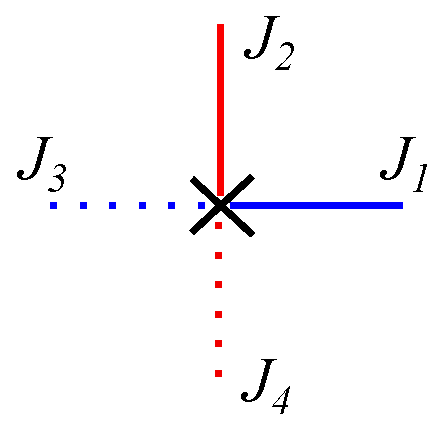
\includegraphics[width=0.7\linewidth]{New_figure/point1.eps} \\ а)}
% 	\end{minipage}
% 	\hfill
% 	\begin{minipage}[h]{0.4\linewidth}
% 		\center{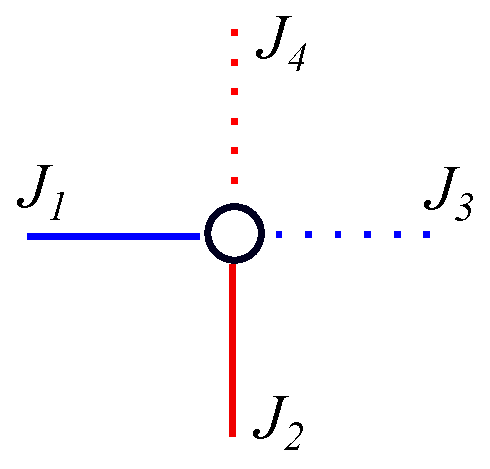
\includegraphics[width=0.7\linewidth]{New_figure/point2.eps} \\ б)}
% 	\end{minipage}
% 	\caption{Два вида узлов на обобщенной квадратной решетке }
% 	\label{point}
% \end{figure}

В связи с этим, в отличие от обычной квадратной решетки, имеем 8 различных направлений на обобщенной квадратной решетке (рисунок \ref{dirgen}): 4 направления из узла , обозначенного кружком (вверх, вниз, влево, вправо) и 4 направления из узла, обозначенного крестом (вверх, вниз, влево, вправо).

% \begin{figure}[h]
% 	\center{\includegraphics[width=0.9\linewidth]{New_figure/dirgen.eps}}
% 	\caption{Возможные направления на обобщенной квадратной решетке}
% 	\label{dirgen}
% \end{figure}

Так же как и в случае обычной квадратной решетки, введем матрицу коэффициентов $\Lambda$, рекурсивные уравнения можно записать в виде
\begin{equation}
W_{r+1}(i, j, \mu) = \sum_{i^{'},\; j^{'},\; \mu^{'}} \Lambda (ij\mu\; |\; i^{'}j^{'}\mu^{'}) W_{r} (i^{'}, j^{'}, \mu^{'}),
\end{equation}

Поскольку существует восемь возможных направлений для движения по решетке, $\Lambda$ представляет собой матрицу $8 \times 8$ с индексами $\mu^{'}$ и $\mu$, графическая интерпретация которой показана на рисунке \ref{matxgen}. 

% \begin{figure}[h]
% 	\center{\includegraphics[width=0.9\linewidth]{New_figure/matxgen.eps}}
% 	\caption{Матричные элементы $\Lambda$}
% 	\label{matxgen}
% \end{figure}

Однако, стоит заметить, что оказывается матрица $\Lambda$ имеет более простой вид, отличный от представленного на рисунке  \ref{matxgen}. Так как у нас не существует направлений движения, при котором из узла, обозначенного кружком, мы бы попадали в такой же узел и, также, у нас не существует направлений движения, при котором из узла, обозначенного крестом, мы бы попадали в похожий узел, поэтому все эти матричные элементы будут равны нулю.

Принимая это во внимание, запишем окончательный вид матрицы коэффициентов $\Lambda$ для обобщенной квадратной решетки в следующем виде

\begin{multline}
\Lambda (p, q, \mu\; |\; p, q, \mu^{'}) = \\ =
\begin{pmatrix}
0 \!\!\!& 0 \!\!\!& 0 \!\!\!& 0\!\!\! & v \epsilon^{-p} \!\!\!& u \alpha^{-1} \epsilon^{-q} \!\!\!& 0 \!\!\!& t \alpha \epsilon^{q} \!\!\! \\
0 \!\!\!& 0 \!\!\!& 0 \!\!\!& 0 \!\!\!& v \alpha \epsilon^{-p}\!\!\! & u \epsilon^{-q}\!\!\! & w \alpha^{-1} \epsilon^{p}\!\!\! & 0\!\!\! \\
0 \!\!\!& 0 \!\!\!& 0 \!\!\!& 0\!\!\! & 0\!\!\! & u \alpha \epsilon^{-q} \!\!\!& w \epsilon^{p} \!\!\!& t \alpha^{-1} \epsilon^{q}\!\!\!  \\
0 \!\!\!& 0 \!\!\!& 0 \!\!\!& 0\!\!\! & v \alpha^{-1} \epsilon^{-p}\!\!\! & 0 \!\!\!& w \alpha \epsilon^{p} \!\!\!& t \epsilon^{q}\!\!\!  \\
w \epsilon^{-p} \!\!\!& t \alpha^{-1} \epsilon^{-q} \!\!\!& 0\!\!\! & u \alpha \epsilon^{q}\!\!\! & 0\!\!\! & 0\!\!\! & 0\!\!\! & 0\!\!\!  \\
w \alpha \epsilon^{-p}\!\!\! & t \epsilon^{-q} \!\!\!& v \alpha^{-1} \epsilon^{p}\!\!\! & 0 \!\!\!& 0\!\!\! & 0\!\!\! & 0\!\!\! & 0\!\!\! \\
0 \!\!\!& t \alpha \epsilon^{-q}\!\!\! & v \epsilon^{p} \!\!\!& u \alpha^{-1} \epsilon^{q}\!\!\! & 0 \!\!\!& 0\!\!\! & 0\!\!\! & 0 \!\!\! \\
w \alpha^{-1} \epsilon^{-p}\!\!\! & 0\!\!\! & v \alpha \epsilon^{p}\!\!\! & u \epsilon^{q} \!\!\!& 0\!\!\! & 0\!\!\! & 0 \!\!\!& 0 \!\!\!
\end{pmatrix},
\end{multline}
где $\epsilon = e^{2\pi i/L}$ и $\alpha = e^{i\pi/4}$.

Следуя алгоритму комбинаторного метода и производя несложные вычисления, имеем точное аналитическое решение обобщенной модели Изинга на квадратной решетке 
\begin{multline}
\ln \frac{\lambda_g}{2} = \frac{1}{16 \pi^2} \int_{0}^{2\pi} \int_{0}^{2\pi} \ln \bigg[\frac{1}{2} \bigg( \ch 2K_1 \ch 2K_2 \ch 2K_3 \ch 2K_4 + \\
+ \sh 2K_1 \sh 2K_2 \sh 2K_3 \sh 2K_4 + 1 - \sh 2K_1 \sh 2K_3 \cos (\omega_1 + \omega_2)  - \\ - \sh 2 K_2 \sh 2 K_4 \cos (\omega_1 - \omega_2)  - (\sh 2 K_1 \sh 2 K_4 + \sh 2 K_2 \sh 2 K_3) \cos \omega_1  - \\ - (\sh 2 K_1 \sh 2 K_2 + \sh 2 K_3 \sh 2 K_4) \cos \omega_2 \bigg) \bigg] d\omega_1 d\omega_2,
\end{multline}
($K_1 = J_1/T$, $K_2 = J_2/T$, $K_3 = J_3/T$, $K_4 = J_4/T$). 

После чего, термодинамические параметры системы, такие как свободная энергия, энтропия и теплоемкость, находятся без труда уже по известным формулам термодинамики \eqref{eq:1.13}, \eqref{eq:1.15}, \eqref{eq:1.16} соответственно.

\section{Термодинамические и фрустрационные особенности обобщенной модели Изинга на квадратной решетке}

Рассмотрим случай, при котором три взаимодействия в решетке являются ферромагнитными, а четвертое --- антиферромагнитное (например, $J_1 = 1$, $J_2 = 1$, $J_3 = 1$, $J_4 = -1$). Аналогичные результаты можно получить при трех антиферромагнитных взаимодействиях и одном ферромагнитном (например, $J_1 = -1$, $J_2 = -1$, $J_3 = -1$, $J_4 = 1$).

При таком выборе обменных взаимодействий энтропия оказывается не равной нулю, а равна некоторому значению --- состояние фрустрировано.  Значение нуль-температурной энтропии было найдено и оно выражается в виде частного двух математических констант
\begin{equation}
S_{T\rightarrow 0} = \frac{G}{\pi} = 0.29156\dots,
\label{g}
\end{equation} 
где $G$ --- постоянная Каталана, важнейшая константа в теории чисел и в комбинаторике.

Температурная зависимость энтропии при $J_1 = 1$, $J_2 = 1$, $J_3 = 1$, \mbox{$J_4 = -1$} приведена на рисунке \ref{ent1} пунктирной линией. 

% \begin{figure}[h]
% 	\center{\includegraphics[width=0.7\linewidth]{New_figure/ent1.eps}}
% 	\caption{Температурные зависимости энтропий для различных параметров обменных взаимодействий: пунктирная кривая --- $J_1 = 1$, $J_2 = 1$, $J_3 = 1$, $J_4 = -1$, желтая кривая --- $J_1 = 1$, $J_2 = 1$ , $J_3 = 1$, $J_4 = -2$, красная кривая --- $J_1 = 1$, $J_2 = 1$ , $J_3 = 1$, $J_4 = -3$, синяя кривая --- $J_1 = 1$, $J_2 = 1$, $J_3 = 1$, $J_4 = -5$, оранжевая кривая --- $J_1 = 1$, $J_2 = 1$ , $J_3 = 1$, $J_4 = -7$, зеленая кривая --- $J_1 = 1$, $J_2 = 1$ , $J_3 = 1$, $J_4 = -8$}
% 	\label{ent1}
% \end{figure}

Начнем увеличивать (по модулю) значение антиферромагнитного взаимодействия $J_4$, оставляя другие взаимодействия без изменений. Температурные зависимости энтропий для некоторых значений обменных взаимодействий проиллюстрированы на рисунке \ref{ent1}. При этом видно, что все приведенные температурные зависимости энтропий имеют одно общее значение при $T \rightarrow 0$. Можно заметить, что при увеличении значения антиферромагнитного взаимодействия $J_4$ график энтропии становится все более и более пологим. 

Установлено, что нуль-температурное значение для энтропий выражается в виде    
\begin{equation}
S_{T\rightarrow 0} = \frac{3}{4\pi} \Cl_2 \bigg(\frac{2\pi}{3}\bigg)   = 0.16153\dots, 
\label{cl}
\end{equation} 
где  $\Cl_2 (\varphi)$ --- функция Клаузена. Функция Клаузена --- трансцендентная специальная функция одной переменной, которая связана с мнимой частью дилогарифма $\Li_2(z)$
\begin{equation*}
\Cl_2 (\varphi) = \im (\Li_2 (e^{i \varphi})) = \im (\Li_2 (i)).
\end{equation*}

Кроме того, функция Клаузена может быть записана через различные интегральные представления, которые можно найти в математическом справочниках и статьях (например, \cite{abramowitz_stegun1972, wood1968}).

Интересно то, что постоянную Каталана так же можно выразить через функцию Клаузена~\cite{wood1968}
\begin{equation*}
G = \Cl_2 \bigg(\frac{\pi}{2}\bigg),
\end{equation*}

% \begin{figure}[h]
% 	\center{\includegraphics[width=0.7\linewidth]{New_figure/heat1.eps}}
% 	\caption{Температурные зависимости теплоемкостей для различных параметров обменных взаимодействий:  пунктирная кривая --- $J_1 = 1$, $J_2 = 1$, $J_3 = 1$, $J_4 = -1$, желтая кривая --- $J_1 = 1$, $J_2 = 1$ , $J_3 = 1$, $J_4 = -2$, красная кривая --- $J_1 = 1$, $J_2 = 1$ , $J_3 = 1$, $J_4 = -3$, синяя кривая --- $J_1 = 1$, $J_2 = 1$, $J_3 = 1$, $J_4 = -5$, оранжевая кривая --- $J_1 = 1$, $J_2 = 1$ , $J_3 = 1$, $J_4 = -7$, зеленая кривая --- $J_1 = 1$, $J_2 = 1$ , $J_3 = 1$, $J_4 = -8$}
% 	\label{heat1}
% \end{figure}

% \begin{figure}[h]
% 	\center{\includegraphics[width=0.8\linewidth]{New_figure/ent2.eps}}
% 	\caption{Температурные зависимости энтропий для различных параметров обменных взаимодействий: фиолетовая кривая --- $J_1 = 1$, $J_2 = 1$, $J_3 = 1$, $J_4 = -9$, желтая кривая --- $J_1 = 1$, $J_2 = 1$, $J_3 = 1$, $J_4 = -10$, красная кривая --- $J_1 = 1$, $J_2 = 1$, $J_3 = 1$, $J_4 = -12$, синяя кривая --- $J_1 = 1$, $J_2 = 1$, $J_3 = 1$, $J_4 = -14$, оранжевая кривая --- $J_1 = 1$, $J_2 = 1$, $J_3 = 1$, $J_4 = -16$}
% 	\label{ent2}
% \end{figure}

% \begin{figure}[H]
% 	\center{\includegraphics[width=0.8\linewidth]{New_figure/heat2.eps}}
% 	\caption{Температурные зависимости теплоемкостей для различных параметров обменных взаимодействий: фиолетовая кривая --- $J_1 = 1$, $J_2 = 1$, $J_3 = 1$, $J_4 = -9$, желтая кривая --- $J_1 = 1$, $J_2 = 1$, $J_3 = 1$, $J_4 = -10$, красная кривая --- $J_1 = 1$, $J_2 = 1$, $J_3 = 1$, $J_4 = -12$, синяя кривая --- $J_1 = 1$, $J_2 = 1$, $J_3 = 1$, $J_4 = -14$, оранжевая кривая --- $J_1 = 1$, $J_2 = 1$, $J_3 = 1$, $J_4 = -16$}
% 	\label{heat2}
% \end{figure}

\noindent поэтому фрустрационное значение энтропии в выражении \eqref{g} может быть переписано в виде
\begin{equation}
\frac{G}{\pi} = \frac{1}{\pi} \Cl_2 \bigg(\frac{\pi}{2}\bigg) = 0.29156\dots
\end{equation}

Поведение теплоемкости при $J_1 = 1$, $J_2 = 1$, $J_3 = 1$, $J_4 = -1$ показано на рисунке \ref{heat1} пунктирной линией. Для остальных температурных зависимостей теплоемкостей их поведение можно объяснить следующим образом. При увеличении значения $J_4$ (по модулю) пик теплоемкости, смещаясь вправо, увеличивается при $J_1 = 1$, $J_2 = 1$, $J_3 = 1$, $J_4 = -2$, после чего пик начинает растягиваться и происходит формирование малого дополнительного пика уже при $J_1 = 1$, $J_2 = 1$, $J_3 = 1$, $J_4 = -5$.

Дальнейшее рассмотрение этого случая показывает, что при увеличении (по модулю) антиферромагнитного взаимодействия $J_4$, сохраняя без изменения $J_1$, $J_2$ и $J_3$, значение у всех нуль-температурных энтропий остается одинаковым и равным \eqref{cl}.

Что касается теплоемкостей (рисунок \ref{heat2}), то положение малого дополнительного пика совершенно не изменяется, что в принципе не характерно обыкновенным фрустрированным системам. Между тем, при увеличении $J_4$ большой широкий пик смещается в правую часть. 

Теперь рассмотрим поведение системы при приближении к точке фрустрации с обменными взаимодействиями $J_1 = 1$, $J_2 = 1$, $J_3 = 1$, $J_4 = -1$. Начнем с параметров $J_1 = 1$, $J_2 = 1$, $J_3 = 1$, $J_4 = 0$. Известно, что при таком выборе взаимодействий реализуется случай гексагональной решетки. Энтропия и теплоемкость гексагональной решетки изображены фиолетовой кривой на рисунках \ref{ent3} и \ref{heat3} соответственно. Будем уменьшать параметр $J_4$ от $0$ до $-0.7$. Глядя на рисунки \ref{ent3} и \ref{heat3}, можно сделать сразу несколько выводов. Во-первых, зависимости теплоемкостей изображены в виде $\Lambda$ - образных пиков. Это значит, что в точках, где теплоемкость испытывает скачок, имеет место фазовый переход. Следовательно, в этих точках не наблюдается бесконечного числа конфигураций с одинаковой энергией, иначе говоря, фрустрации отсутствуют. Во-вторых, при приближении к точке фрустрации $J_1 = 1$, $J_2 = 1$, $J_3 = 1$, $J_4 = -1$ зависимости теплоемкостей, смещаясь влево по температуре, испытывают укручение левой части графика. 

% \begin{figure}[H]
% 	\center{\includegraphics[width=0.65\linewidth]{New_figure/ent3.eps}}
% 	\caption{Температурные зависимости энтропий для различных параметров обменных взаимодействий: фиолетовая кривая --- $J_1 = 1$, $J_2 = 1$, $J_3 = 1$, $J_4 = 0$, желтая кривая --- $J_1 = 1$, $J_2 = 1$, $J_3 = 1$, $J_4 = -0.1$, красная кривая --- $J_1 = 1$, $J_2 = 1$, $J_3 = 1$, $J_4 = -0.2$, синяя кривая --- $J_1 = 1$, $J_2 = 1$, $J_3 = 1$, $J_4 = -0.3$, оранжевая кривая --- $J_1 = 1$, $J_2 = 1$, $J_3 = 1$, $J_4 = -0.4$, зеленая кривая --- $J_1 = 1$, $J_2 = 1$, $J_3 = 1$, $J_4 = -0.5$, розовая кривая --- $J_1 = 1$, $J_2 = 1$, $J_3 = 1$, $J_4 = -0.6$, темно-зеленая кривая --- $J_1 = 1$, $J_2 = 1$, $J_3 = 1$, $J_4 = -0.7$}
% 	\label{ent3}
% \end{figure}

% \begin{figure}[H]
% 	\center{\includegraphics[width=0.65\linewidth]{New_figure/heat3.eps}}
% 	\caption{Температурные зависимости теплоемкостей для различных параметров обменных взаимодействий: фиолетовая кривая --- $J_1 = 1$, $J_2 = 1$, $J_3 = 1$, $J_4 = 0$, желтая кривая --- $J_1 = 1$, $J_2 = 1$, $J_3 = 1$, $J_4 = -0.1$, красная кривая --- $J_1 = 1$, $J_2 = 1$, $J_3 = 1$, $J_4 = -0.2$, синяя кривая --- $J_1 = 1$, $J_2 = 1$, $J_3 = 1$, $J_4 = -0.3$, оранжевая кривая --- $J_1 = 1$, $J_2 = 1$, $J_3 = 1$, $J_4 = -0.4$, зеленая кривая --- $J_1 = 1$, $J_2 = 1$, $J_3 = 1$, $J_4 = -0.5$, розовая кривая --- $J_1 = 1$, $J_2 = 1$, $J_3 = 1$, $J_4 = -0.6$, темно-зеленая кривая --- $J_1 = 1$, $J_2 = 1$, $J_3 = 1$, $J_4 = -0.7$}
% 	\label{heat3}
% \end{figure}

% \begin{figure}[H]
% 	\center{\includegraphics[width=0.7\linewidth]{New_figure/ent4.eps}}
% 	\caption{Температурные зависимости энтропий для различных параметров обменных взаимодействий: фиолетовая кривая --- $J_1 = 1$, $J_2 = 1$, $J_3 = 1$, $J_4 = 0$, желтая кривая --- $J_1 = 1$, $J_2 = 1$, $J_3 = 1$, $J_4 = 1$, красная кривая --- $J_1 = 1$, $J_2 = 1$, $J_3 = 1$, $J_4 = 2$, синяя кривая --- $J_1 = 1$, $J_2 = 1$, $J_3 = 1$, $J_4 = 5$, оранжевая кривая --- $J_1 = 1$, $J_2 = 1$, $J_3 = 1$, $J_4 = 7$, зеленая кривая --- $J_1 = 1$, $J_2 = 1$, $J_3 = 1$, $J_4 = 12$}
% 	\label{ent4}
% \end{figure}

% \begin{figure}[H]
% 	\center{\includegraphics[width=0.7\linewidth]{New_figure/heat4.eps}}
% 	\caption{Температурные зависимости теплоемкостей для различных параметров обменных взаимодействий: фиолетовая кривая --- $J_1 = 1$, $J_2 = 1$, $J_3 = 1$, $J_4 = 0$, желтая кривая --- $J_1 = 1$, $J_2 = 1$, $J_3 = 1$, $J_4 = 1$, красная кривая --- $J_1 = 1$, $J_2 = 1$, $J_3 = 1$, $J_4 = 2$, синяя кривая --- $J_1 = 1$, $J_2 = 1$, $J_3 = 1$, $J_4 = 5$, оранжевая кривая --- $J_1 = 1$, $J_2 = 1$, $J_3 = 1$, $J_4 = 7$, зеленая кривая --- $J_1 = 1$, $J_2 = 1$, $J_3 = 1$, $J_4 = 12$}
% 	\label{heat4}
% \end{figure}

При увеличении взаимодействия $J_4$, начиная от $0$, можно получить еще один частный случай. Подтверждением этого служат рисунки \ref{ent4} и \ref{heat4}. Видно, что при больших значениях $J_4$ графики как энтропий, так и теплоемкостей сходятся к некоторой точке перехода. Это ни что иное как температура перехода для треугольной решетки. Ведь при стремлении одного из взаимодействий в бесконечность, обобщенная квадратная решетка сводится к треугольной решетке. На рисунках \ref{ent4} и \ref{heat4} фиолетовыми кривыми указаны энтропия и теплоемкость гексагональной решетки, желтыми кривыми --- для квадратной решетки, зелеными кривыми --- для треугольной решетки.

\section{Частные случаи обобщенной модели Изинга на квадратной решетке}

\subsection{Обычная квадратная решетка}
 
Если положить, что $J_1 = J_3$ и $J_2 = J_4$, то обобщенная модель Изинга на квадратной решетке сводится к обычной модели Изинга на квадратной решетке. Решение обычной модели Изинга было подробно исследовано в Главе 1. Также, мы увидели, что квадратная решетка при любых параметрах обменного взаимодействия в отсутствие магнитного поля не является фрустрированной.

% \begin{figure}[h]
%     \center{\includegraphics[width=0.5\linewidth]{New_figure/dual1.png}}
%     \caption{Самодуальность квадратной решетки~\cite{mussardo2010}}
%     \label{dual1}
% \end{figure}

Кроме того, квадратная решетка является самодуальной, то есть она дуальна сама себе~(рисунок~\ref{dual1}). Температура перехода --- $T_c^{square} = J\cdot 2.2692\dots$.

\subsection{Треугольная решетка} 

Переход от обобщенной квадратной решетки к треугольной осуществляется при стремлении одного взаимодействия к бесконечности. На рисунке \ref{triag} мы устремляли к бесконечности обменное взаимодействие $J_1$.  

Точное решение для треугольной решетки можно получить комбинаторным методом Вдовиченко--Фейнмана. 
Матрица коэффициентов $\Lambda$ треугольной решетки может быть записана в виде
\begin{multline}
\Lambda (p, q, \mu\; |\; p, q, \mu^{'}) = \\ =
\begin{pmatrix}
y \epsilon^{-p} & x \alpha^{-1} \epsilon^{-p-q}  &  z \alpha^{-2} \epsilon^{-q}  &  0  &  x \alpha^2 \epsilon^{p+q}  &  z \alpha \epsilon^{q} \\
y \alpha \epsilon^{-p} & x \epsilon^{-p-q}  &  z \alpha^{-1} \epsilon^{-q}  &  y \alpha^{-2} \epsilon^{p}  &  0  &  z \alpha^2 \epsilon^{q} \\
y \alpha^2 \epsilon^{-p} & x \alpha \epsilon^{-p-q}  &  z \epsilon^{-q}  &  y \alpha^{-1} \epsilon^{p}  &  x \alpha^{-2} \epsilon^{p+q}  &  0 \\
0 & x \alpha^{2} \epsilon^{-p-q}  &  z \alpha \epsilon^{-q}  &  y \epsilon^{p}  &  x \alpha^{-1} \epsilon^{p+q}  &  z \alpha^{-2} \epsilon^{q} \\
y \alpha^{-2} \epsilon^{-p} & 0  &  z \alpha^{2} \epsilon^{-q}  &  y \alpha \epsilon^{p}  &  x \epsilon^{p+q}  &  z \alpha^{-1} \epsilon^{q} \\
y \alpha^{-1} \epsilon^{-p} & x \alpha^{-2} \epsilon^{-p-q}  &  0  &  y \alpha^{2} \epsilon^{p}  &  x \alpha \epsilon^{p+q}  &  z \epsilon^{q} \\
\end{pmatrix},
\end{multline}
где $x = \th K_1$, $y = \th K_2$, $z = \th K_3$, $\epsilon = e^{2\pi i/L}$ и $\alpha = e^{i\pi/6}$.

Воспроизводя алгоритм комбинаторного метода Вдовиченко--Фейнмана, описанный в Главе 1, получаем точное решение модели Изинга на треугольной решетке~\cite{wannier1950}
\begin{multline}
\ln \frac{\lambda_t}{2} = \frac{1}{8 \pi^2} \int_{0}^{2\pi} \int_{0}^{2\pi} \ln \bigg[ \ch 2K_1 \ch 2K_2 \ch 2K_3  + \sh 2K_1 \sh 2K_2 \sh 2K_3 - \\ - \sh 2K_2 \cos (\omega_1 + \omega_2)  -  \sh 2 K_3 \cos \omega_1  - \sh 2 K_1 \cos \omega_2 \bigg] d\omega_1 d\omega_2,
\end{multline}
($K_1 = J_1/T$, $K_2 = J_2/T$, $K_3 = J_3/T$). 

Рассмотрим подлогарифмическое выражение при $J_1 = J_2 = J_3 = J$ и $\omega_1 = \omega_2 = 0$, тогда
\begin{equation}
\ch^3 \bigg(\frac{2J}{T_c} \bigg) + \sh^3\bigg(\frac{2J}{T_c}\bigg) - 3 \sh \bigg(\frac{2J}{T_c}\bigg) = 0.
\label{lab}
\end{equation}

Решая уравнение \eqref{lab} относительно $T_c$, получим температуру перехода треугольной решетки
\begin{align}
T_c^{triangle} &= 4J/\ln 3;& T_c^{triangle} &= J\cdot 3.64096\dots.
\end{align}

Как мы уже знаем, треугольная решетка допускает наличие фрустрационных состояний, а именно, при $J_1 = J_2 = J_3 = -1$. Однако, нуль-температурное значение энтропии, известное из статьи~\cite{wannier1950} и записанное в выражении~\eqref{wannier}, может быть переписано через функцию Клаузена как
\begin{equation}
S_{T\rightarrow 0} = \frac{1}{\pi} \Cl_2 \bigg(\frac{\pi}{3}\bigg).
\end{equation}

Дуальной к треугольной решетке является гексагональная решетка и наоборот~(рисунок~\ref{dual2}).

% \begin{figure}[h]
% 	\center{\includegraphics[width=0.85\linewidth]{New_figure/dual2.png}}
% 	\caption{Дуальные друг к другу решетки: треугольная и гексагональная решетки~\cite{mussardo2010}}
% 	\label{dual2}
% \end{figure}

\subsection{Гексагональная решетка}

Для получения гексагональной решетки из обобщенной квадратной решетки необходимо приравнять любое из четырех обменных взаимодействий нулю. Получим решетку типа «кирпичная кладка», которая в свою очередь топологически эквивалентна гексагональной решетке (рисунок \ref{hex}).

Точное решение для гексагональной решетки так же может быть получено комбинаторным методом Вдовиченко--Фейнмана. Матрица коэффициентов $\Lambda$ для гексагональной решетки имеет следующий вид
\begin{multline}
\Lambda (p, q, \mu\; |\; p, q, \mu^{'}) = \\ =
\begin{pmatrix}
0 & 0  & 0  & x \alpha^{-1} \epsilon^{-p}  & 0  & z \alpha \epsilon^{p+q} \\
0 & 0  & 0  & x \alpha \epsilon^{-p}  & y \alpha^{-1} \epsilon^{-q}  & 0 \\
0 & 0  & 0  & 0  & y \alpha \epsilon^{-q}  & z \alpha^{-1} \epsilon^{p+q} \\
y \alpha \epsilon^{q} & z \alpha^{-1} \epsilon^{-p-q}  & 0  & 0  & 0  & 0 \\
0 & z \alpha \epsilon^{-p-q}  & x \alpha^{-1} \epsilon^p  & 0  & 0  & 0 \\
y \alpha^{-1} \epsilon^{q} & 0  & x \alpha \epsilon^p  & 0  & 0  & 0 
\end{pmatrix},
\end{multline}
где $x = \th K_1$, $y = \th K_2$, $z = \th K_3$, $\epsilon = e^{2\pi i/L}$ и $\alpha = e^{i\pi/6}$.

Производя соответствующие расчеты, получаем точное аналитическое решение модели Изинга на гексагональной решетке~\cite{houtapell1950}
\begin{multline}
\ln \frac{\lambda_h}{2} = \frac{1}{16 \pi^2} \int_{0}^{2\pi} \int_{0}^{2\pi} \ln \bigg[\frac{1}{2} \bigg( \ch 2K_1 \ch 2K_2 \ch 2K_3 + 1 \\ - \sh 2 K_1 \sh 2 K_3 \cos (\omega_1 - \omega_2)  - \sh 2 K_1 \sh 2 K_2 \cos \omega_1  - \\ - \sh 2 K_2 \sh 2 K_3 \cos \omega_2 \bigg) \bigg] d\omega_1 d\omega_2,
\end{multline}
($K_1 = J_1/T$, $K_2 = J_2/T$, $K_3 = J_3/T$). 


Рассмотрим подлогарифмическое выражение при $J_1 = J_2 = J_3 = J$ и $\omega_1 = \omega_2 = 0$, тогда
\begin{equation}
\frac{1}{2}\bigg(\ch^3 \bigg(\frac{2J}{T_c} \bigg) + 1 - 3 \sh \bigg(\frac{2J}{T_c}\bigg)\bigg) = 0.
\label{lab1}
\end{equation}

Решив уравнение \eqref{lab1}, получим температуру перехода для гексагональной решетки
\begin{align}
T_c^{hex} &= \frac{2J}{\ln (2 + \sqrt{3})};& T_c^{hex} &= J \cdot 1.51865\dots.
\end{align}

Гексагональная решетка, как и квадратная решетка, не является фрустрированной при любых параметрах обменных взаимодействий в отсутствие магнитного поля. Таким образом, это значит, что на гексагональной решетке можно расположить спины так, чтобы каждая пара ближайших соседей была антипараллельна.

\subsection{Другие виды решеток}

При равенстве двух обменных взаимодействий нулю, реализуется случай обобщенной модели Изинга на одномерной цепочке, который был подробно исследован в Главе 2.

Если все взаимодействия, кроме одного, оказываются равными нулю, то задача сводится к случаю решетки димеров, так же рассмотренных в Главе 2.

\FloatBarrier